\chapter{Input Point or Finite-fault Sources}\label{chapter-source}

Seismic wave is actived by the seimisc source.
In seismic wave equations, the seismic source is represented by the force term ($\mathbf{F}$)
 and/or stress gluss term ($\mathbf{\dot{\mathbf{M}}}$) at the right-hand side (RHS) of the equations:
\begin{align}
   \rho \frac{\partial \mathbf{v}}{\partial t} &= \nabla \cdot \mathbf{\sigma} + \mathbf{F}, \\
   \frac{\partial \sigma}{\partial t} &= \mathbf{C} : \frac{1}{2} \left( \nabla \mathbf{v} + \mathbf{v} \nabla \right) - \dot{\mathbf{M}}.
\end{align}
The force term is used for sources acting as an external force to the simulatin region,
while the stress gluss term could be used to implement a general moment tensor souce.
It is relative easy to implement the source in the code by adding the respective terms onto the RHS values.
We just need a way to input different combinations of how many sources, the locations, source time funcion (STF) and source mechanism
for a single simulation into the code.


Different applications may require a source in different formats, e.g,
\begin{enumerate}
    \item single force at a single point, which is a common source for Green function and exploration seismology;
    \item general moment source at a single point, which is used for small earthquake and explosive source;
    \item general moment sources along a fault, which is also called finite-fault source model and used for large earthquake;
    \item time-reversed waveforms along surface, which is used for time reversal imaging;
    \item plane wave incident for teleseismic wave problems.
\end{enumerate}
The first two sources act at a single point, while the last three types are implemented by adding many single point sources simultaneously 
along a fault, a surface or a pre-defined line (plane). The first two types can be taken as a special case of the last three types
when number of the source becomes one.


The CGFD3D package tries to implement different sources to support different applications.
Thus we allow to input a single point source or many point sources.
For easy usage, we also support:
\begin{itemize}
    \item the location of the single point could be grid index or coordinate;
    \item the vertical coordinate could be given by the absolute axis or the depth relative the free surface (to be done!);
    \item STF of each single point source could be an analytical wavelet function or discrete values obtained by real data inversion or source dynamic simulation;
    \item the source could be a force source and/or a moment one;
    \item the  moment source could be given by the six tensor components or the mechanism angles plus $\mu DA$.
\end{itemize}


To allow different input combinations of above different parameters, 
we use several flags in the input file to determine the specific input meaning of the related parameters.
In the following, we will describe the format of the source input file of the CGFD3D package
 and give several examples to show how to input different sources.


%=============================================================
\section{Set Parameters in Main Par File} \label{src_json}
%=============================================================

All the detailed specification of the source is written in a separate source file (.src).
Throug the main input .json file, we need to tell the simulation code where is the source file,
which is specified by \verb|in_source_file|.
There are total three paramters in the .json file related to the source input:
\begin{itemize}
  \item \verb|in_source_file|: \\
     set the input source file;
  \item \verb|is_export_source|: \\
     determine if export the internal discreted source for QC (not implemented yet);
  \item \verb|source_export_dir|: \\
     the path for source exporting.
\end{itemize}
Currently, only \verb|in_source_file| is implemented and the other two have no effect yet.

\begin{lstlisting}[language=json, title=Example of source settings in .json, frame=tb]
   "in_source_file" : "/home/user/prj/input/test.src",
   "is_export_source" : 1,
   "source_export_dir" : "/home/user/prj/output",
\end{lstlisting}


%===================================================================
\section{Set Source Information by the Source Input File (.src)} \label{src_format}
%=============================================================

The .src file is designed to input all the required source information using different representations.
Considering parallel computing using MPI on a multi-nodes cluster, we want to allocate
large array holdding discrete STF values for only the source located at the node.
Thus we divide the information in the .src into three regions (line number refer that in the example):
\begin{enumerate}
    \item global information related to all the sources (line 1-20);
    \item location information of each source (line 21-25);
    \item STF and component information of each source (after line 26).
\end{enumerate}
In other words, we specify the global information/flags first,
 then list the locations of all the sources,
 and finally give the STF and component values of each source.
 The last part may be very large for discrete STF input.
%\begin{enumerate}
%    \item meta data: name (or id) of the this source input, number of sources, locations of each source;
%    \item value data: source time function or values, source mechansims, etc.
%\end{enumerate}

A sample .src file using analytical wavelet function as STF is shown below.
 We will use this sample .src file to explain the file format of .src file.
\begin{lstlisting}[language=bash, caption=Source input file using analytical wavelet,
   numbers=left, numbersep=5pt,numberstyle=\tiny\color{codegray}, commentstyle=\color{codegreen},
   frame=tb]
# name of this input source
event_1
# number of source
1
# flag for stf
#  1st value : 0 analytic stf or 1 discrete values
#    for analytical, 2nd value is time length
#    for discrete,  2nd value is dt and 3rd is nt
#    e.g.,
# 0 4.0 
# 1 0.05 20
0 1.0
# flag for source component and mechanism format
#  1st value: source components, 1(force), 2(momoment), 3(force+moment)
#  2nd value: mechanism format for moment source:
#       0 : 6 moment components, 
#       1 : 3 angles, mu, slip rate or D, A (mu <0 means to use internal mu value)
2 0
# flag for location
#   1st value: meaning of the location: 0 computational coordinate, 1 physical coordinate
#   2nd value: 0 absolute axis or 1 depth relative to the free surface of the third coordinate
1 0
# location of each source
#   sx sy sz
#80 49 50
#80 49 50
8020 4930 -950
# stf and cmp
0.0 ricker 2.0 0.5   # t0  stf_name  ricker_fc ricker_t0
1e16  1e16  1e16 0 0 0 
\end{lstlisting}


From above sample file, We see that we can insert comment line in the .src file using "\#" as the line start, similar to the Bash script syntax.
What we should set in the .src file are:
\begin{itemize}
    \item name of the whole source (represented by EVTNM, following sac notation) (line 2), type should be string without whitespace.
        This name is used for output file naming.
        E.g., the output sac file will start with "event\_1" for this sample file.
    \item number of the sources (NS) (line 4), type is interger.
         The second part should contain NS locations and the third part should contains NS STF and cmp settings.
    \item settings about STF (line 12). Two values or three values depends on the first value,
        which tells the code how STF is given (STF\_flag): 
        \begin{itemize}
        \item 0: the STF whill be set using wavelet name and related coefficiences in the second part for each source.
              The second value here sets the same total time length of all the STF 
              to reduce using computer memory to hold discrete STF in simulation.
        \item 1: the STF will be given as discrete values.
              Then the second value is the time step (stf\_dt) and the third one is the total number of time step (stf\_nt).
        \end{itemize}
        We should note that in the third part, we will give each source a separte start time to implement finite-fault source combining
        above time window setting.
    \item two values to set force and/or moment type of each source, and how the moment source is given (line 16).
        The first value (CMP\_flag):
        \begin{itemize}
            \item 1: force;
            \item 2: moment;
            \item 3: force and momemnt.
        \end{itemize}
        The second value (Mechanism\_flag) determines how the mechanism is given if moment source is used:
        \begin{itemize}
            \item 0: values of the six components of the moment tensor;
            \item 1: strke, dip and rake angels, plus $\mu$, $D$, and $A$.$\mu$ <0 means to use internal $\mu$ value.
        \end{itemize}
    \item two flags about the meaning of the location values (line 20).
        The first flag is the meaning of the location (LOC\_flag), 
        \begin{itemize}
            \item 0: the location is given by the computational coordinate. The value is same to the grid index in this implementation. 
                The decimal part is the relative shift of the source to the grid point;
            \item 1: the location is given as the physical coordinate values, which is the Cartesian coordinate in this implementation.
        \end{itemize}
        The second flag (Vertical\_flag) is used when the first flag set 1 to determine the third coordinate is
        \begin{itemize}
            \item 0: absolute z-axis value;
            \item 1: depth relative to the free surface (need to be implemented!).
        \end{itemize}
    \item Then the second part, the locations of each sources (line 22-25). There should be NS lines for NS sources.
        Each line contains three values representing the location of one source.
        If LOC\_flag = 0 (computational coordinate), the location should be given by grid index with decimal as
\begin{lstlisting}[language=bash, caption=Source location by computational coordinate,
   numbers=left, numbersep=5pt,numberstyle=\tiny\color{codegray}, commentstyle=\color{codegreen},
   frame=tb]
# location of each source (e.g., for NS = 3)
20.0 20.0 50.0
30.0 29.0 50.0
40.5 50.2 55.1
\end{lstlisting}
        If LOC\_flag = 1 (physical coordinate), the location should be given by its coordinate values as
\begin{lstlisting}[language=bash, caption=Source location by physical coordinate,
   numbers=left, numbersep=5pt,numberstyle=\tiny\color{codegray}, commentstyle=\color{codegreen},
   frame=tb]
# location of each source (e.g., for NS = 3)
2000.0 2000.0 5000.0
3000.0 2900.0 5000.0
4050.0 5020.0 5510.0
\end{lstlisting}
    \item The third part specifies STF and component values of each source (after line 26).
        The formats are different for different STF\_flag. \\
        If STF\_flag = 0 (wavelet name), each source has two lines,
        \begin{enumerate}
            \item two or more values to set the STF:
            \begin{itemize}
                \item first value: the activated (or start) time, which is important for finite-fault model to represent fault rupture.
                \item second value: a string, the wavelet function name.
                      The valid wavelet names for current CGFD3D are shown in table~\ref{table_wavelet}
                      (more wavelent functions will be implemented in the future). You can easily add a wavelet by modifying function
                      \verb|src_cal_wavelet| in src\_t.c.
                \item 3rd-12th values: the coefficients required by the wavelet function.
                      Different wavelet may require different number of coefficients.
                      Here we allow up to maximum 10 coefficients to specify the values.
                      It will no problem only setting one or two values if the wavelet only needs one or two coefficients.
                      Please see table~\ref{table_wavelet} for the number and meanings of coefficients of current supported wavelets.
            \end{itemize}
            \item 3, 6 or 9 values (depending on CMP\_flag) to give the magnitudes of the force and/or moment components.
                \begin{itemize}
                    \item CMP\_flag=1: 3 values to set values of $F_x$ $F_y$ and $F_z$;
                    \item CMP\_flag=2: 6 values to set values of the moment tensor, ordered as 
                        \begin{itemize}
                            \item $m_{xx},m_{yy},m_{zz},m_{yz},m_{xz},m_{xy}$ following the 
                                  Viogt nonation (Fig~\ref{fig_voigt}) if Mechanism\_flag=0
                            \item strike, dip, rake, $\mu, D, A$ if Mechanism\_flag=1.
                        \end{itemize}
                    \item CMP\_flag=3: 9 values to set values of both the force and the moment tensor, ordered as 
                        \begin{itemize}
                            \item $F_x,F_y,F_z,m_{xx},m_{yy},m_{zz},m_{yz},m_{xz},m_{xy}$ if Mechanism\_flag=0
                            \item $F_x,F_y,F_z$, strike, dip, rake, $\mu, D, A$ if Mechanism\_flag=1.
                        \end{itemize}
                \end{itemize}
        \end{enumerate}

        If STF\_flag = 1 (discrete values), each source has (1+stf\_nt) lines (see sample Listing~\ref{lst_stf_value}),
        \begin{enumerate}
            \item first line: one value, the activated (or start) time.
            \item stf\_nt lines of 3, 6 or 9 values (depending on CMP\_flag) to give the magnitudes of the force and/or moment components at each time step:
                \begin{itemize}
                    \item CMP\_flag=1: 3 values of $F_x$ $F_y$ and $F_z$;
                    \item CMP\_flag=2: 6 values of the moment tensor, ordered as 
                        \begin{itemize}
                            \item $m_{xx},m_{yy},m_{zz},m_{yz},m_{xz},m_{xy}$ following the 
                                  Viogt nonation (Fig~\ref{fig_voigt}) if Mechanism\_flag=0
                            \item strike, dip, rake, $\mu, D, A$ if Mechanism\_flag=1.
                        \end{itemize}
                    \item CMP\_flag=3: 9 values of both the force and the moment tensor, ordered as 
                        \begin{itemize}
                            \item $F_x,F_y,F_z,m_{xx},m_{yy},m_{zz},m_{yz},m_{xz},m_{xy}$ if Mechanism\_flag=0
                            \item $F_x,F_y,F_z$, strike, dip, rake, $\mu, D, A$ if Mechanism\_flag=1.
                        \end{itemize}
                \end{itemize}
        \end{enumerate}
\end{itemize}


\begin{table}[h!]
\centering
\caption{Implemented Wavelet functions and their coefficients.}
\label{table_wavelet}
\begin{tabular}{| c | c | c |}
\hline
   wavelet name  &   coef[0]    &   coef[1] \\
\hline
    ricker        &   cetral frequency  &  central time shift \\
\hline
   ricker\_deriv  &   cetral frequency  &  central time shift \\
\hline
    gaussian      &    RMS value  &  time shift \\
\hline
  gaussian\_deriv  &   RMS value  &  time shift \\
\hline
\end{tabular}
\end{table}


\begin{figure}
    \centering
    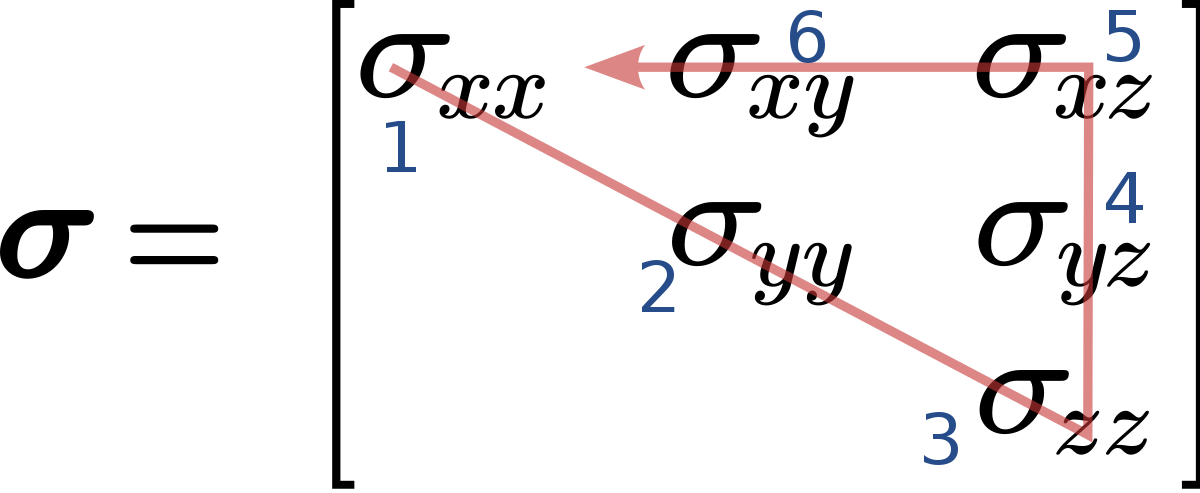
\includegraphics[width=0.5\textwidth]{Voigt_notation_Mnemonic_rule_svg.png}
    \caption{Viogt notation (From: \href{https://en.wikipedia.org/wiki/Voigt_notation}{Wiki})}
    \label{fig_voigt}
\end{figure}


\begin{lstlisting}[language=bash, caption=Source input file using discrete STF, label={lst_stf_value},
   numbers=left, numbersep=5pt,numberstyle=\tiny\color{codegray}, commentstyle=\color{codegreen},
   frame=single]
# name_of_this_input_src
evt_1_stf_value
# number of source
1
# meaning of the location: 0 computational coordinate, 1 physical coordinate
#     axis or depth of the third coordinate: 0 axis, 1 depth
0 1
# stf_input_type and time length info
#  0 4.0 : analytic and time window length of each stf
#  1 0.05 20  : 1 value and time_step num_of_step
1 0.025 40
# 1(force) 2(momoment) 3(force+moment)
#    mechanism type for moment source: 0 moment, 1 angle + mu + D + A
2 0
# meta data of each source
#   sx sy sz
80 49 50
# value data for each source
#  t0
0.0 
# Mxx etc
4.29488e+12    4.29488e+12   4.29488e+12     0.0  0.0  0.0
1.0088e+13     1.0088e+13    1.0088e+13      0.0  0.0  0.1
2.24061e+13    2.24061e+13   2.24061e+13     0.0  0.0  0.0
4.70162e+13    4.70162e+13   4.70162e+13     0.0  0.0  0.0
9.31041e+13    9.31041e+13   9.31041e+13     0.0  0.0  0.0
1.73751e+14    1.73751e+14   1.73751e+14     0.0  0.0  0.0
3.05036e+14    3.05036e+14   3.05036e+14     0.0  0.0  0.0
5.02611e+14    5.02611e+14   5.02611e+14     0.0  0.0  0.0
7.7483e+14     7.7483e+14    7.7483e+14      0.0  0.0  0.0
1.11265e+15    1.11265e+15   1.11265e+15     0.0  0.0  0.0
1.47863e+15    1.47863e+15   1.47863e+15     0.0  0.0  0.0
1.79991e+15    1.79991e+15   1.79991e+15     0.0  0.0  0.0
1.97157e+15    1.97157e+15   1.97157e+15     0.0  0.0  0.0
1.87557e+15    1.87557e+15   1.87557e+15     0.0  0.0  0.0
1.41548e+15    1.41548e+15   1.41548e+15     0.0  0.0  0.0
5.58831e+14    5.58831e+14   5.58831e+14     0.0  0.0  0.0
-6.2831e+14    -6.2831e+14   -6.2831e+14     0.0  0.0  0.0
-1.97263e+15   -1.97263e+15  -1.97263e+15    0.0  0.0  0.0
-3.22222e+15   -3.22222e+15  -3.22222e+15    0.0  0.0  0.0
-4.1098e+15    -4.1098e+15   -4.1098e+15     0.0  0.0  0.0
-4.43113e+15   -4.43113e+15  -4.43113e+15    0.0  0.0  0.0
-4.1098e+15    -4.1098e+15   -4.1098e+15     0.0  0.0  0.0
-3.22222e+15   -3.22222e+15  -3.22222e+15    0.0  0.0  0.0
-1.97263e+15   -1.97263e+15  -1.97263e+15    0.0  0.0  0.0
-6.28308e+14   -6.28308e+14  -6.28308e+14    0.0  0.0  0.0
5.58831e+14    5.58831e+14   5.58831e+14     0.0  0.0  0.0
1.41548e+15    1.41548e+15   1.41548e+15     0.0  0.0  0.0
1.87557e+15    1.87557e+15   1.87557e+15     0.0  0.0  0.0
1.97157e+15    1.97157e+15   1.97157e+15     0.0  0.0  0.0
1.79991e+15    1.79991e+15   1.79991e+15     0.0  0.0  0.0
1.47863e+15    1.47863e+15   1.47863e+15     0.0  0.0  0.0
1.11265e+15    1.11265e+15   1.11265e+15     0.0  0.0  0.0
7.7483e+14     7.7483e+14    7.7483e+14      0.0  0.0  0.0
5.02611e+14    5.02611e+14   5.02611e+14     0.0  0.0  0.0
3.05036e+14    3.05036e+14   3.05036e+14     0.0  0.0  0.0
1.73751e+14    1.73751e+14   1.73751e+14     0.0  0.0  0.0
9.3104e+13     9.3104e+13    9.3104e+13      0.0  0.0  0.0
4.70162e+13    4.70162e+13   4.70162e+13     0.0  0.0  0.0
2.24061e+13    2.24061e+13   2.24061e+13     0.0  0.0  0.0
1.0088e+13     1.0088e+13    1.0088e+13      0.0  0.0  0.0
\end{lstlisting}
